\documentclass[12pt,en,a4paper]{article}
\usepackage[utf8]{inputenc}
\usepackage{anyfontsize}
\usepackage{pifont}
\usepackage{enumerate}
\usepackage{lastpage}
\usepackage{caption}
\usepackage{color}
\usepackage{natbib}
\usepackage{graphicx}
\usepackage{fancyhdr}
\usepackage{float}
\usepackage{tikz}
\usepackage[framemethod=tikz]{mdframed}
\usepackage{listings}
\usetikzlibrary{calc,backgrounds}
\newcommand\HRule{\rule{12cm}{1pt}}
\pagestyle{fancy}
\fancyhead{} % clear all header fields
\fancyhead[L]{
	\color{blue}
	\begin{tabular}{rl}
		\begin{picture}(25,15)(0,0)
		\put(0,-8){
\includegraphics[width=8mm, height=8mm]{BK.png}}
		\end{picture}
		\begin{tabular}{l}
			\textbf{\bf \ttfamily Ho Chi Minh University of Technology}\\
			\textbf{\bf \ttfamily Faculty of Computer Science \& Engineering}
		\end{tabular} 	
	\end{tabular}
}
\fancyhead[R]{
	\begin{tabular}{l}
		\tiny \bf \\
		\tiny \bf 
	\end{tabular}
}
\fancyfoot{} % clear all footer fields
\fancyfoot[L]{\scriptsize \ttfamily Matlab Project 191}
\fancyfoot[R]{\scriptsize \ttfamily Page {\thepage}/\pageref{LastPage}}
\renewcommand{\headrulewidth}{0.3pt}
\renewcommand{\footrulewidth}{0.3pt}

\definecolor{dkgreen}{rgb}{0,0.6,0}
\definecolor{gray}{rgb}{0.5,0.5,0.5}
\definecolor{mauve}{rgb}{0.58,0,0.82}

\lstset{frame=tb,
	language=Matlab,
	aboveskip=3mm,
	belowskip=3mm,
	showstringspaces=false,
	columns=flexible,
	basicstyle={\small\ttfamily},
	numbers=none,
	numberstyle=\tiny\color{gray},
	keywordstyle=\color{blue},
	commentstyle=\color{dkgreen},
	stringstyle=\color{mauve},
	breaklines=true,
	breakatwhitespace=true,
	tabsize=3,
	numbers=left,
	stepnumber=1,
	numbersep=1pt,    
	firstnumber=1,
	numberfirstline=true
}

\begin{document}
	\begin{titlepage}
		
\begin{tikzpicture}[remember picture, overlay]
		\draw[line width = 2pt] ($(current page.north west) + (1in,-1in)$) rectangle ($(current page.south east) + (-1in,1in)$);
		\end{tikzpicture}
		
		\begin{center}
			
			% Upper part of the page
			\textbf{\fontsize{12pt}{1pt}\selectfont HO CHI MINH CITY UNIVERSITY OF TECHNOLOGY}\\[0.5cm]
			{\fontsize{13pt}{1pt}\selectfont Faculty of Computer Science \& Engineering}\\[0.5cm]
			\begin{figure}[h]
				\centering
				
\includegraphics[width=1.7in,height=1.7in]{BK.png}
			\end{figure}
			
			% Title
			\HRule \\[0.5cm]
			{ \textbf{\fontsize{25pt}{1pt}\selectfont MATLAB PROJECT 191}}\\[0.4cm]
			
			\HRule \\[0.8cm]
			\begin{minipage}{0.545\textwidth}   
				\begin{flushleft} 
					\textbf{Authors:}\\
					Vu Anh Nhi - 1952380\\
					Huynh Nhat Quang - 1952112\\
					Dinh Huy Thien - 1952462\\
					Hoang Nhu Ngoc - 1911697\\
					Tran Nguyen Anh Khoa - 1911419\\
					Trinh Quang Tien - 1952133\\
					Nguyen Thanh Ngan - 1911667\\
					Nguyen Chinh Khoi - 1952793\\
					Nguyen Hoang - 1952255\\
					Nguyen Khuong - 1952310\\
				\end{flushleft}
			\end{minipage}
			\begin{minipage}{0.4\textwidth}
				\begin{flushright} 
					\textbf{Class:}\\
					MT1004\\
					\textbf{Lecturer:}\\
					Dau The Phiet\\
					
				\end{flushright}
			\end{minipage}
			
			\vfill
			
			% Bottom of the page
			\vspace{2cm}
			{\large \today}
		\end{center}
	\end{titlepage}
	
	\section*{Problem 1}
	For each of the functions f below, approximate its derivative at the given value x = a in two different ways. First, use a computer microscope (i.e., a graphing program) to view the graph of f near x = a. Zoom in until the graph appears straight and find its slope. Second, use a calculator to find the values of the quotient
	\[ 
	\frac{f(a+h)-f(a-h)}{2h}
	\]
	for h = .1, .01, .001, ..., .000001. Based on these values of the quotients, give your best estimate for f'(a), and say how many decimal places of accuracy it has.\par
	\subsection*{About using computer microscope:}
	\begin{itemize}
		\item Firstly, we sketch the graph of the given function, then we zoom in at the point \(x = a\) until the graph appears to be a straight line. Take two points A and B (Let A be on the left and B on the right) on the graph in that region and calculate the slope using the following formula:
		\[Slope=\frac{y_{B}-y_{A}}{x_{B}-x_{A}}\]
	\end{itemize}
	\begin{enumerate}[a)]
		\item \(f(x)=\frac{1}{x}\) at \(x=2\)
	\end{enumerate}
	\begin{itemize}
		\item Using a calculator gives us the answer -0.25
		\item Using the following codes gives us this graph
		\begin{mdframed}[hidealllines=true,backgroundcolor=magenta!10]
			\begin{lstlisting}
			syms x;
			y=1/x;
			fplot(y);
			xlim([1.9 2.1]);
			ylim([0.45 0.55]);
			hold on;
			plot(1.92, 1/1.92, '*r');
			text(1.92, 0.528, 'X: 1.92');
			text(1.92, 0.524, 'Y: 0.52');
			plot(2.08, 1/2.08, '*r');
			text(2.06, 0.478, 'X: 2.06');
			text(2.06, 0.474, 'Y: 0.48');
			plot(2, 1/2, '*r');
			text(1.9975, 0.496, 'A');
			hold off;
			\end{lstlisting}
		\end{mdframed}
		\begin{figure}[!h]
			\centering
			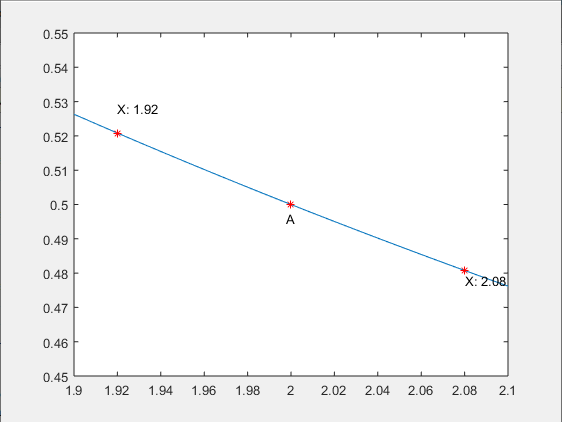
\includegraphics[scale=0.5]{1a.png}
			\caption*{Problem 1a}
			\label{prob1a}
		\end{figure}
		\item Using these codes to estimate \(f'(a)\) (df in this case means \(f'(a)\))\\
		\begin{mdframed}[hidealllines=true,backgroundcolor=magenta!10]
			\begin{lstlisting}
			syms x df h;
			h = input('h = ');
			df = (1./(2+h) - 1./(2-h))/(2.*h);
			format long;
			df
			\end{lstlisting}
		\end{mdframed}
		\item And we have the result table
		\begin{table}[h]
			\centering
			\begin{tabular}{|l|l|}
				\hline
				h & \(f'(a)\) \\ \hline
				0.1 & -0.250626566416040 \\ \hline
				0.01 & -0.250006250156248 \\ \hline
				0.001 & -0.250000062499978 \\ \hline
				0.0001 & -0.250000000625583 \\ \hline
				0.00001 & -0.250000000009964 \\ \hline
				0.000001 & -0.249999999979433 \\ \hline
				0.0000001 & -0.249999999868411 \\ \hline
			\end{tabular}
		\end{table}
		\item The best estimation is -0.250000000009964 when h = 0.00001 and it has 13 decimal places of accuracy.
	\end{itemize}
	\begin{enumerate}[b)]
		\item \(sin(7x)\) at \(x=3\)
	\end{enumerate}
	\begin{itemize}
		\item Using a calculator gives us the answer -3.834104822
		\item Using the following codes gives us this graph\\
		\begin{mdframed}[hidealllines=true,backgroundcolor=magenta!10]
			\begin{lstlisting}
			syms x;
			y=sin(7*x);
			fplot(y);
			xlim([2.99 3.01]);
			ylim([0.797 0.872]);
			hold on;
			plot(3, sin(21), '*r');
			text(2.9998, 0.834, 'A');
			plot(2.994, sin(7*2.994), '*r');
			text(2.994, 0.865, 'X: 2.994');
			plot(3.006, sin(7*3.006), '*r');
			text(3.006, 0.819, 'X: 3.006');
			hold off;
			\end{lstlisting}
		\end{mdframed}
		\begin{figure}[h]
			\centering
			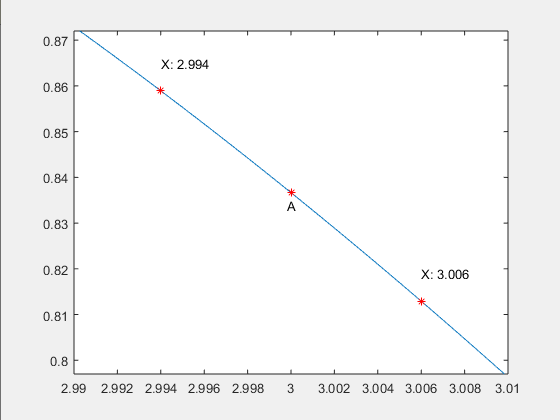
\includegraphics[scale=0.5]{1b.png}
			\caption*{Problem 1b}
			\label{prob1b}
		\end{figure}
		\item Using these codes to estimate \(f'(a)\) (df in this case means \(f'(a)\))\\
		\begin{mdframed}[hidealllines=true,backgroundcolor=magenta!10]
			\begin{lstlisting}
			syms x df h;
			h = input('h = ');
			df = (sin(7*(3+h))-sin(7*(3-h)))/(2.*h);
			format long;
			df
			\end{lstlisting}
		\end{mdframed}
		\item And we have the result table
		\begin{table}[!h]
			\centering
			\begin{tabular}{|l|l|}
				\hline
				h & \(f'(a)\) \\ \hline
				0.1 & -3.528568772540893 \\ \hline
				0.01 & -3.830974403016590 \\ \hline
				0.001 & -3.834073509789426 \\ \hline
				0.0001 & -3.834104508461667 \\ \hline
				0.00001 & -3.834104818489780 \\ \hline
				0.000001 & -3.834104821576201 \\ \hline
				0.0000001 & -3.834104807531880 \\ \hline
			\end{tabular}
		\end{table}
		\item The best estimation is -3.834104821576201 when h = 0.000001 and it has 10 decimal places of accuracy.
	\end{itemize}
	\begin{enumerate}[c)]
		\item \(x^{3}\) at \(x=200\)
	\end{enumerate}
	\begin{itemize}
		\item Using a calculator gives us the answer 120000
		\item Using the following codes gives us this graph\\
		\begin{mdframed}[hidealllines=true,backgroundcolor=magenta!10]
			\begin{lstlisting}
			syms x;
			y=x\textasciicircum3;
			fplot(y);
			xlim([199.999 200.001]);
			ylim([7999999 8000001]);
			hold on;
			plot(200, 200, '*r');
			text(200.00004, 200, 'A');
			plot(200.000007, 200.000007, '*r');
			text(200.00004, 200.000007, 'X: 200 + 7E-6');
			plot(199.999993, 199.999993, '*r');
			text(200.00003, 199.9999935, 'X: 200 - 7E-6');
			hold off;
			\end{lstlisting}
		\end{mdframed}
		\begin{figure}[h]
			\centering
			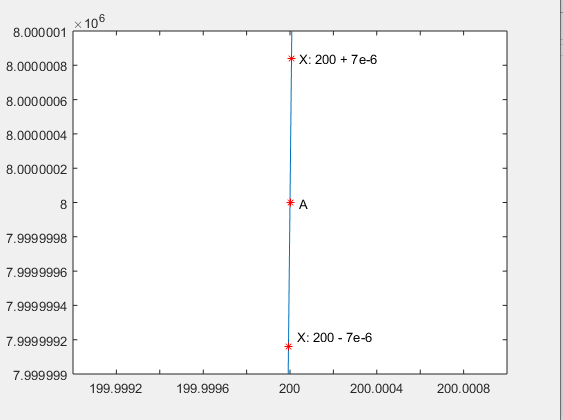
\includegraphics[scale=0.5]{1c.png}
			\caption*{Problem 1c}
			\label{prob1c}
		\end{figure}
		\item Use these codes to estimate \(f'(a)\) (df in this case means \(f'(a)\))\\
		\begin{mdframed}[hidealllines=true,backgroundcolor=magenta!10]
			\begin{lstlisting}
			syms x df h;
			h = input('h = ');
			df = ((200+h)\textasciicircum3 - (200-h)\textasciicircum3)/(2.*h);
			format long;
			df
			\end{lstlisting}
		\end{mdframed}
		\item And we have the result table
		\begin{table}[h]
			\centering
			\begin{tabular}{|l|l|}
				\hline
				h & \(f'(a)\) \\ \hline
				0.1 & 1.200000099999923e+05 \\ \hline
				0.01 & 1.200000000998844e+05 \\ \hline
				0.001 & 1.200000000018627e+05 \\ \hline
				0.0001 & 1.200000000046566e+05 \\ \hline
				0.00001 & 1.200000000651926e+05 \\ \hline
				0.000001 & 1.199999996460974e+05 \\ \hline
				0.0000001 & 1.199999917298555e+05 \\ \hline
			\end{tabular}
		\end{table}
		\item The best estimation is 1.200000000018627E+5 when h = 0.001 and it has 12 decimal places of accuracy.
	\end{itemize}
	\begin{enumerate}[d)]
		\item \(2^{x}\) at \(x=5\)
	\end{enumerate}
	\begin{itemize}
		\item Using Wolfram Alpha gives us the answer 22.18070977791824990135
		\item Using the following codes gives us this graph
		\begin{mdframed}[hidealllines=true,backgroundcolor=magenta!10]
			\begin{lstlisting}
			syms x;
			y=2\textasciicircum x;
			fplot(y);
			xlim([4.99 5.01]);
			ylim([31.75 32.25]);
			hold on;
			plot(5, 2\textasciicircum5, '*r');
			text(5, 31.98, 'A');
			plot(4.992, 2\textasciicircum4.992, '*r');
			text(4.992, 31.81, 'X: 4.992');
			plot(5.008, 2\textasciicircum5.008, '*r');
			text(5.0073, 32.15, 'X: 5.008');
			hold off;
			\end{lstlisting}
		\end{mdframed}
		\begin{figure}[h]
			\centering
			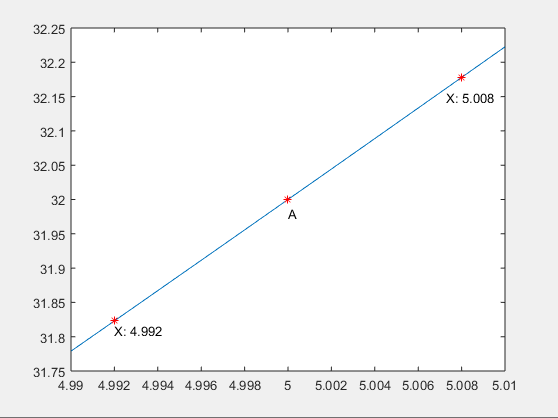
\includegraphics[scale=0.5]{1d.png}
			\caption*{Problem 1d}
			\label{prob1d}
		\end{figure}
		\item Using these codes to estimate \(f'(a)\) (df in this case means \(f'(a)\))\\
		\begin{mdframed}[hidealllines=true,backgroundcolor=magenta!10]
			\begin{lstlisting}
			syms x df h;
			h = input('h = ');
			df = (2\textasciicircum(5+h) - 2\textasciicircum(5-h))/(2.*h);
			format long;
			df
			\end{lstlisting}
		\end{mdframed}
		\item And we have the result table
		
		\begin{table}[h]
			\centering
			\begin{tabular}{|l|l|}
				\hline
				0.1 & 22.198475359917644 \\ \hline
				0.01 & 22.180887391492199 \\ \hline
				0.001 & 22.180711554058874 \\ \hline
				0.0001 & 22.180709795645015 \\ \hline
				0.00001 & 22.180709777153137 \\ \hline
				0.000001 & 22.180709779107133 \\ \hline
				0.0000001 & 22.180709837726909 \\ \hline
			\end{tabular}
		\end{table}
		\item The best estimated is 22.180709777153137 when x=0.00001 and it has 12 decimal places of accuracy.
	\end{itemize}
	\newpage
	\section*{Problem 2}
	\textbf{How to approximate definite integral:}\\
	We apply the following equation: \[\int_{a}^{b}f(x)dx\approx \sum_{i=1}^{n}f(x_{i}^{*})\Delta x\] where \(\Delta x=\frac{b-a}{n}\) and \(x_{i}^{*}\) lies in interval \([x_{i-1},x_{i}]\).
	\begin{itemize}
		\item If we choose \(x_{i}^{*}\) to be the left endpoint of interval [$x_{i-1}$,$x_i$], then this approximation is called Left Endpoint Approximation:  \[\int_{a}^{b}f(x)dx\approx \sum_{i=1}^{n}f(x_{i-1})\Delta x\]
		\item If we choose \(x_{i}^{*}\) to be the right endpoint of interval [$x_{i-1}$,$x_i$], then this approximation is called Right Endpoint Approximation: \[\int_{a}^{b}f(x)dx\approx \sum_{i=1}^{n}f(x_{i})\Delta x\]
		\item If we choose \(x_{i}^{*}\) to be the midpoint of interval [$x_{i-1}$,$x_i$], then this approximation is called Midpoint Approximation: \[\int_{a}^{b}f(x)dx\approx \sum_{i=1}^{n}f(\frac{1}{2}(x_{i-1}+x_{i}))\Delta x\]
	\end{itemize}
	\begin{enumerate}[a)]
		\item \(\int_{1}^{2}\frac{1}{x}dx\), divide [1,2] into 10 and 20 subsintervals.
	\end{enumerate}
	\begin{itemize}
		\item Divide [1,2] into 10 subsintevals, we have \(\Delta x=\frac{2-1}{10}=0.1\)
		\item {[1,2]} is divided into 10 subsintervals: [1,1.1], [1.1,1.2],…, [1.9,2]
		\item Use Left Endpoint Approximation:
		\[\int_{1}^{2}\frac{1}{x}dx\approx (f(1)+f(1.1)+...+f(1.9))0.1=(\frac{1}{1}+\frac{1}{1.1}+...+\frac{1}{1.9})0.1\]
		\begin{itemize}
			\item Codes based on the rules:\\
			\begin{mdframed}[hidealllines=true,backgroundcolor=magenta!10]
				\begin{lstlisting}
				x = 1:0.1:1.9;
				y = 0.1./x;
				disp(sum(y));
				\end{lstlisting}
			\end{mdframed}
			\item The result is 0.7188
		\end{itemize}
		\item Use Right Endpoint Approximation:
		\[\int_{1}^{2}\frac{1}{x}dx\approx (f(1.1)+f(1.2)+...+f(2))0.1=(\frac{1}{1.1}+\frac{1}{1.2}+...+\frac{1}{2})0.1\]
		\begin{itemize}
			\item Codes based on the rules:\\
			\begin{mdframed}[hidealllines=true,backgroundcolor=magenta!10]
				\begin{lstlisting}
				x = 1.1:0.1:2;
				y = 0.1./x;
				disp(sum(y));
				\end{lstlisting}
			\end{mdframed}
			\item The result is 0.6688
		\end{itemize}
		\item Use Midpoint Approximation:
		\[\int_{1}^{2}\frac{1}{x}dx\approx (f(1.05)+f(1.15)+...+f(1.95))0.1=(\frac{1}{1.05}+\frac{1}{1.15}+...+\frac{1}{1.95})0.1\]
		\begin{itemize}
			\item Codes based on the rules:\\
			\begin{mdframed}[hidealllines=true,backgroundcolor=magenta!10]
				\begin{lstlisting}
				x = 1.05:0.1:1.95;
				y = 0.1./x;
				disp(sum(y));
				\end{lstlisting}
			\end{mdframed}
			\item The result is 0.6928
		\end{itemize}
		\item Divide [1,2] into 20 subsintevals, we have \(\Delta x=\frac{2-1}{20}=0.05\)
		\item {[1,2]} is divided into 20 subsinterval: [1,1.05], [1.05,1.1],…, [1.95,2]
		\item Use Left Endpoint Approximation:
		\[\int_{1}^{2}\frac{1}{x}dx\approx (f(1)+f(1.05)+...+f(1.95))0.05=(\frac{1}{1}+\frac{1}{1.05}+...+\frac{1}{1.95})0.05\]
		\begin{itemize}
			\item Code based on the rules:\\
			\begin{mdframed}[hidealllines=true,backgroundcolor=magenta!10]
				\begin{lstlisting}
				x = 1:0.05:1.95;
				y = 0.1./x;
				disp(sum(y));
				\end{lstlisting}
			\end{mdframed}
			\item The result is 0.7058
		\end{itemize}
		\item Use Right Endpoint Approximation:
		\[\int_{1}^{2}\frac{1}{x}dx\approx (f(1.05)+f(1.1)+...+f(2))0.05=(\frac{1}{1.05}+\frac{1}{1.1}+...+\frac{1}{2})0.05\]
		\begin{itemize}
			\item Code based on the rules:\\
			\begin{mdframed}[hidealllines=true,backgroundcolor=magenta!10]
				\begin{lstlisting}
				x = 1.05:0.05:2;
				y = 0.1./x;
				disp(sum(y));
				\end{lstlisting}
			\end{mdframed}
			\item The result is 0.6808
		\end{itemize}
		\item Use Midpoint Approximation
		\[\int_{1}^{2}\frac{1}{x}dx\approx (f(1.025)+f(1.075)+...+f(1.95))0.05=(\frac{1}{1.025}+\frac{1}{1.075}+...+\frac{1}{1.975})0.05\]
		\begin{itemize}
			\item Code based on the rules:\\
			\begin{mdframed}[hidealllines=true,backgroundcolor=magenta!10]
				\begin{lstlisting}
				x = 1.025:0.05:1.975;
				y = 0.1./x;
				disp(sum(y));
				\end{lstlisting}
			\end{mdframed}
			\item The result is 0.6931
		\end{itemize}
	\end{itemize}
	\begin{enumerate}[b)]
		\item \(\int_{0}^{2}e^{-x^{2}}\), divide [0,2] into 10 and 20 subsintervals.
	\end{enumerate}
	\begin{itemize}
		\item Divide [0,2] into 10 subsintevals, we have \(\Delta x=\frac{2-0}{10}=0.2\)
		\item {[0,2]} is divided into 10 subsintervals: [0,0.2], [0.2,0.4],…, [1.8,2]
		\item Use Left Endpoint Approximation:
		\[\int_{0}^{2}e^{-x^{2}}\approx (f(0)+f(0.2)+...+f(1.8))0.2=(e^{-0^{2}}+e^{-0.2^{2}}+...+e^{-1.8^{2}})0.2\]
		\begin{itemize}
			\item Codes based on the rules:\\
			\begin{mdframed}[hidealllines=true,backgroundcolor=magenta!10]
				\begin{lstlisting}
				x = 0:0.2:1.8;
				y = 0.2*exp(-x.*x);
				disp(sum(y));
				\end{lstlisting}
			\end{mdframed}
			\item The result is 0.9800
		\end{itemize}
		\item Use Right Endpoint Approximation:
		\[\int_{0}^{2}e^{-x^{2}}\approx (f(0.2)+f(0.4)+...+f(2))0.2=(e^{-0.2^{2}}+e^{-0.4^{2}}+...+e^{-2^{2}})0.2\]
		\begin{itemize}
			\item Codes based on the rules:\\
			\begin{mdframed}[hidealllines=true,backgroundcolor=magenta!10]
				\begin{lstlisting}
				x = 0.2:0.2:2;
				y = 0.2*exp(-x.*x);
				disp(sum(y));
				\end{lstlisting}
			\end{mdframed}
			\item The result is 0.7837
		\end{itemize}
		\item Midpoint Approximation
		\[\int_{0}^{2}e^{-x^{2}}\approx (f(0.1)+f(0.3)+...+f(1.9))0.2=(e^{-0.1^{2}}+e^{-0.3^{2}}+...+e^{-1.9^{2}})0.2\]
		\begin{itemize}
			\item Codes based on the rules:\\
			\begin{mdframed}[hidealllines=true,backgroundcolor=magenta!10]
				\begin{lstlisting}
				x = 0.1:0.2:1.9;
				y = 0.2*exp(-x.*x);
				disp(sum(y));
				\end{lstlisting}
			\end{mdframed}
			\item The result is 0.8822
		\end{itemize}
		\item Divide [0,2] into 20 subsintevals, we have \(\Delta x=\frac{2-0}{20}=0.1\)
		\item {[0,2]} is divided into 20 subsintervals: [0,0.1], [0.1,0.2],…, [1.9,2]
		\item Use Left Endpoint Approximation:
		\[\int_{0}^{2}e^{-x^{2}}\approx (f(0)+f(0.1)+...+f(1.9))0.1=(e^{-0^{2}}+e^{-0.1^{2}}+...+e^{-1.9^{2}})0.1\]
		\begin{itemize}
			\item Codes based on the rules:\\
			\begin{mdframed}[hidealllines=true,backgroundcolor=magenta!10]
				\begin{lstlisting}
				x = 0:0.1:1.9;
				y = 0.2*exp(-x.*x);
				disp(sum(y));
				\end{lstlisting}
			\end{mdframed}
			\item The result is 0.9311
		\end{itemize}
		\item Use Right Endpoint Approximation:
		\[\int_{0}^{2}e^{-x^{2}}\approx (f(0.1)+f(0.2)+...+f(2))0.1=(e^{-0.1^{2}}+e^{-0.2^{2}}+...+e^{-2^{2}})0.1\]
		\begin{itemize}
			\item Codes based on the rules:\\
			\begin{mdframed}[hidealllines=true,backgroundcolor=magenta!10]
				\begin{lstlisting}
				x = 0.1:0.1:2;
				y = 0.2*exp(-x.*x);
				disp(sum(y));
				\end{lstlisting}
			\end{mdframed}
			\item The result is 0.8329
		\end{itemize}
		\item Midpoint Approximation
		\[\int_{0}^{2}e^{-x^{2}}\approx (f(0.05)+f(0.15)+...+f(1.95))0.1=(e^{-0.05^{2}}+e^{-0.15^{2}}+...+e^{-1.95^{2}})0.1\]
		\begin{itemize}
			\item Codes based on the rules:\\
			\begin{mdframed}[hidealllines=true,backgroundcolor=magenta!10]
				\begin{lstlisting}
				x = 0.05:0.1:1.95;
				y = 0.2*exp(-x.*x);
				disp(sum(y));
				\end{lstlisting}
			\end{mdframed}
			\item The result is 0.8821
		\end{itemize}
	\end{itemize}
	\newpage
	\section*{Problem 3}
	Study the Euler method to approximate the solution of first order differential equations. The following questions concern a rabbit population described by the logistic model \(R'=0.1R(1-\frac{R}{25000})\) rabbits per month
	\begin{enumerate}[a)]
		\item What happens to a population of 2000 rabbits after 6 months, after 24 months, and after 5 years? To answer each question, present a table of successive approximations that allows you to give the exact value to the nearest whole number.
	\end{enumerate}
	\textbf{How do we apply Euler method?}
	\begin{itemize}
		\item Consider the problem of calculating the shape of an unknown curve which starts at a given point and satisfies a given differential equation. Here, a differential equation can be thought of as a formula by which the slope of the tangent line of the curve can be calculated at any point on the curve, once the position of that point has been defined.
		\item Following by the formula: \(y=y'_{0}(x-x_{0})+y_{0}\), we can calculate \(y'_{0}\) through the differential equation. After we denote \(y’(x) = f(t,y(x))\), \(x – x_{0} = h\), we can find the value of the n-th \(y\) by: \(y_{n}=y_{n-1}+hf(t_{n-1},y_{n-1})s\)
	\end{itemize}
	\begin{itemize}
		\item Using Euler method with an initial population of 2000, the steps h is 0.001 month we have the code:\\
		\begin{mdframed}[hidealllines=true,backgroundcolor=magenta!10]
			\begin{lstlisting}
			f = @(y) 0.1*y*(1- y/25000);
			x0 = 0;
			y0 = 2000;
			xn = 60;
			h = 0.1;
			hold on;
			while x0 <= xn
			y1 = y0 + h * f(y0);
			x1 = x0 + h;
			x0 = x1;
			y0 = y1;
			fprintf('\n%4.3f %4.3f', x0, y0);
			plot(x0, y0, '.');
			end
			hold off;
			\end{lstlisting}
		\end{mdframed}
		\item And the result we receive:
		\begin{table}[h]
			\centering
			\begin{tabular}{lll}
				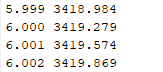
\includegraphics{table1.png}&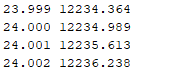
\includegraphics{table2.png}  & 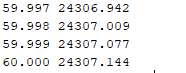
\includegraphics{table3.png}
			\end{tabular}
		\end{table}
		\begin{table}[h]
			\centering
			\begin{tabular}{|l|l|}
				\hline
				R(6)  & 3419.279  \\ \hline
				R(24) & 12234.989 \\ \hline
				R(60) & 24307.144 \\ \hline
			\end{tabular}
		\end{table}
	\end{itemize}
	\begin{enumerate}[b)]
		\item Sketch the functions determined by the logistic equation if you start with either 2000 or 40000 rabbits. Compare the two functions. How do they differ? In what ways are they similar?
	\end{enumerate}
	\begin{itemize}
		\item The code gives us the graph:
		\begin{figure}[h]
			\centering
			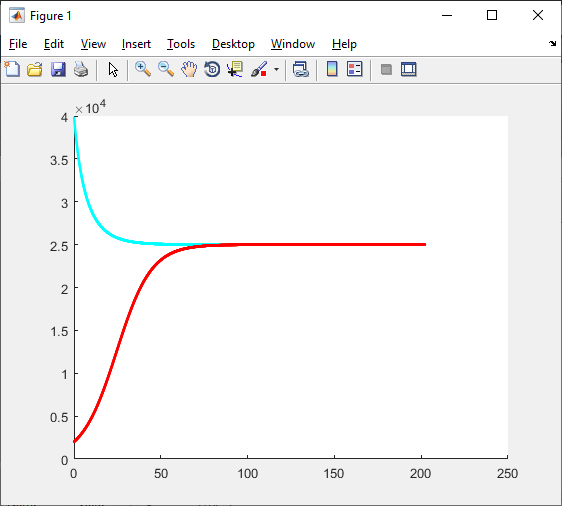
\includegraphics[scale=0.35]{3.png}
			\label{fig:mesh1}
		\end{figure}
		\item Similarity: Both functions move toward the line of 25000 and remain stable.
		\item Difference:
		\begin{table}[H]
			\centering
			\begin{tabular}{|l|l|}
				\hline
				Start at 2000 & The function’s graph tends to increase to 25000 \\ \hline
				Start at 40000 & The function’s graph tends to decrease to 25000 \\ \hline
			\end{tabular}
		\end{table}
	\end{itemize}
\end{document}